\documentclass[tikz,margin=6pt]{standalone}
\usepackage{pgfplots}
\pgfplotsset{compat=1.12}

\begin{document}
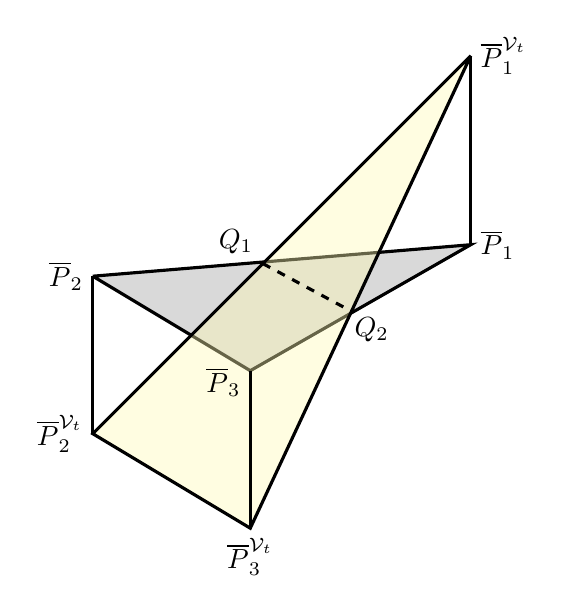
\begin{tikzpicture}[scale=0.8]

\draw[fill=gray!30, line width=0.4mm] (0,1.5) -- (6,2) -- (2.5,0) -- (0,1.5);  % base triangle
\draw[fill=yellow!30, opacity=.4, line width=0.1mm] (6,5) -- (0,-1) -- (2.5,-2.5) -- (6,5);
\draw[line width=0.4mm] (6,5) -- (0,-1) -- (2.5,-2.5) -- (6,5);
% upper triangle
\draw[line width=0.4mm] (0,1.5) -- (0,-1);
\draw[line width=0.4mm] (2.5,0) -- (2.5,-2.5);
\draw[line width=0.4mm] (6,2) -- (6,5);

\node[anchor=east] at (0,1.5) {$\overline{P}_2$};
\node[anchor=north east] at (2.5,0.2) {$\overline{P}_3$};
\node[anchor=west] at (6,2) {$\overline{P}_1$};
\node[anchor=east] at (0,-1) {$\overline{P}_2^{\mathcal{V}_t}$};
\node[anchor=north] at (2.5,-2.5) {$\overline{P}_3^{\mathcal{V}_t}$};
\node[anchor=west] at (6,5) {$\overline{P}_1^{\mathcal{V}_t}$};

\draw[dashed, line width=0.4mm] (2.7,1.7) -- (4,1);

\node[anchor=north west] at (4,1) {$Q_2$};
\node[anchor=south east] at (2.7,1.7) {$Q_1$};

\end{tikzpicture}
\end{document}
